% The Edge Grid -- IEEE conference paper (IEEEtran).
% Build:  tectonic docs/paper-ieee/main.tex   (or: pdflatex main.tex, run twice)
% Content source of truth: docs/paper-ieee.md. Figures: docs/figures/.
\documentclass[conference]{IEEEtran}
\IEEEoverridecommandlockouts
\usepackage{cite}
\usepackage{amsmath,amssymb}
\usepackage{graphicx}
\usepackage{array}
\usepackage{booktabs}
\usepackage[T1]{fontenc}
\usepackage{textcomp}
\usepackage{xcolor}
\usepackage[hidelinks]{hyperref}
\graphicspath{{../figures/}{docs/figures/}}

\newcolumntype{P}[1]{>{\raggedright\arraybackslash}p{#1}}

\begin{document}

\title{The Edge Grid: A Prototype for Decentralized,\\ Verifiable Peer-to-Peer AI Inference}

\author{
\IEEEauthorblockN{Harshit Raj}
\IEEEauthorblockA{\textit{Dept. of CSE (IoT, Cyber-Security}\\ \textit{\& Blockchain Tech.)}\\
\textit{Sir M. Visvesvaraya Inst. of Technology}\\ Bengaluru, India}
\and
\IEEEauthorblockN{Chetan Raghuvanshi}
\IEEEauthorblockA{\textit{Dept. of CSE (IoT, Cyber-Security}\\ \textit{\& Blockchain Tech.)}\\
\textit{Sir M. Visvesvaraya Inst. of Technology}\\ Bengaluru, India}
\and
\IEEEauthorblockN{Keshav Narayan}
\IEEEauthorblockA{\textit{Dept. of CSE (IoT, Cyber-Security}\\ \textit{\& Blockchain Tech.)}\\
\textit{Sir M. Visvesvaraya Inst. of Technology}\\ Bengaluru, India}
\and
\IEEEauthorblockN{Mayur Agarwal}
\IEEEauthorblockA{\textit{Dept. of CSE (IoT, Cyber-Security}\\ \textit{\& Blockchain Tech.)}\\
\textit{Sir M. Visvesvaraya Inst. of Technology}\\ Bengaluru, India}
}

\maketitle

\begin{abstract}
Centralized inference services concentrate pricing power, availability, and trust in a single
operator, and decentralized physical infrastructure networks have already shown that peer-to-peer
markets can sell connectivity, storage, and general compute at scale. Selling verifiable AI
inference the same way raises a problem those networks do not solve: an anonymous edge provider,
operating under a hard latency budget, has both the means and the incentive to return a
plausible-looking wrong answer, and naive redundancy or centralized scheduling cannot detect that
cheaply. We design a network in which a job is discovered and auctioned under a sealed-bid,
warm-start-aware second-price rule; executed by a streaming edge inference runtime; committed to a
Merkle-backed data-availability layer; and verified by a two-tier mechanism that separates a
trustless cryptographic fraud proof from a sampled, quorum-voted semantic judge, with staked
collateral slashed 80/20 between reporter and treasury on confirmed fraud. We build and measure a
small-scale reference implementation on commodity CPU hardware: warm time-to-first-token averaged
610\,ms with a 12$\times$ cold-start penalty; a sealed-bid auction cleared correctly across 57
trials and responded near-linearly to injected per-link network delay; content-addressed model
weights were fetched, independently re-verified, and correctly rejected under three tampering
scenarios; and on-chain settlement conserved value exactly across all three resolution paths. The
verification layer's measured behavior is the paper's central finding: the deployable,
edge-hostable judge configuration caught only 30--35\% of two semantically subtle fraud strategies
while scoring them confidently rather than hesitantly, and a follow-up experiment indicates that
this failure tracks judge capability rather than the judge's relationship to the model it polices,
refuting an explanation this evaluation initially favored.
\end{abstract}

\begin{IEEEkeywords}
decentralized physical infrastructure networks, verifiable AI inference, LLM-as-a-Judge,
second-price auctions, optimistic fraud proofs, staked settlement
\end{IEEEkeywords}

% ---------------------------------------------------------------------------
\section{Introduction}

Centralized inference services have made large-model access cheap and reliable at the cost of
concentrating pricing power, infrastructure control, and data governance in a small number of
operators. Decentralized physical infrastructure networks (DePIN) already sell connectivity,
storage, and general compute competitively; none solve the narrower problem this paper addresses:
\textbf{selling AI inference, rather than raw compute, from anonymous edge providers under a
latency budget, with correctness verified cheaply enough that verification does not eat the
economics it protects.}

Redundant execution multiplies cost by the redundancy factor for every job, not just the audited
fraction, which is economically incompatible with a centralized provider's marginal cost.
Centralized verification reintroduces the single point of control the network exists to remove.
Reputation punishes a \emph{pattern}, not a specific transaction. What is needed is a mechanism
that prices a latency budget at routing time, verifies a \emph{sampled} fraction of jobs cheaply,
and makes fraud's economic consequence automatic, without a central adjudicator. Two properties
make this harder than verifying storage: a wrong answer need not look wrong (a fabricated fact or
negated claim can be fluent and indistinguishable from a correct one), and the party best
positioned to catch a subtle semantic error is itself a language model, so the verification layer
inherits every reliability question that attaches to language models generally, including that it
can be confidently wrong. Section~\ref{sec:verif} is a direct measurement of that risk.

We design the network around a strict separation between two kinds of verification claim. A
\textbf{cryptographic fraud proof} establishes with certainty that a provider served output
inconsistent with what it committed on chain: a fact about two hashes, needing no challenge
period. A \textbf{semantic verdict} is a judgment call about whether a faithfully delivered output
is actually correct, rendered by one or more independent validator models under a quorum rule.
This lets the cheap, certain tier absorb one entire class of dishonesty for a fixed cost, and
confines the expensive, probabilistic tier to the dishonesty that genuinely requires judgment.

\textbf{Design contributions:} (1)~a market protocol combining a sealed-bid second-price auction
with a warm-start handicap applied to ranking score but never to payment, since model residency
measures as a near-eligibility condition rather than a tradeable quality dimension under realistic
latency budgets; (2)~a two-tier verification protocol with a three-valued verdict that never
collapses ``unreachable'' into either a pass or a fraud finding; (3)~settlement as an escrow whose
release requires no privileged party online, with unbonding collateral that stays slashable to
close a front-running window.

\textbf{Prototype and evaluation contributions:} (1)~a working, reproducible reference
implementation with every figure traceable to a configuration-snapshotted run; (2)~measurement
that the deployable verification configuration is confidently wrong on two of four fraud
strategies, and that this tracks judge \emph{capability} rather than \emph{lineage}, refuting an
explanation we initially favored; (3)~measurement that quorum aggregation reduces false positives
well below individual members at no cost to recall; (4)~identification of a methodological
confound: a model-generated ``honest'' control is not reliably honest and bounds every
LLM-as-a-Judge precision figure, a problem that recurred in our own pipeline even after being
diagnosed once.

% ---------------------------------------------------------------------------
\section{Related Work}

\textbf{DePIN networks} already sell compute, storage, or connectivity through token-incentivized
provider sets: Bittensor rewards ML work but allocates reward predominantly by stake rather than
output quality~\cite{bittensor}; Akash~\cite{akash} and Golem~\cite{golem} auction general compute
without an inference-specific verification layer; Gensyn~\cite{gensyn} targets verifiable ML
compute oriented toward training. None couples a latency-bounded auction to a sampled semantic
verification layer with staked slashing.

\textbf{Morpheus}~\cite{morpheus,morpheusnode} is the closest architectural precedent: an
Arbitrum-L2 marketplace where providers bid and contracts match them to serve LLM inference. We
differ in mechanism (a warm-start-aware second-price auction with hard-constraint eligibility) and
in adding a two-tier verification layer outside Morpheus's stated scope. DGrid~\cite{dgrid} and
Parallax~\cite{parallax} describe decentralized inference serving without the auction or
verification layers evaluated here; both are a vendor litepaper and a preprint respectively, not
peer-reviewed. \textbf{PolyLink}~\cite{polylink} is the closest refereed academic parallel for
settlement but does not evaluate an auction's response to injected latency
(Section~\ref{sec:auction}).

Our data-availability layer implements the \emph{binding} property of fraud and
data-availability proofs~\cite{albassam} against a local store, explicitly declining their
\emph{availability} guarantee. Settlement's challenge-window structure follows the fraud-proof
lineage established for rollups~\cite{arbitrum,albassam,truebit}. The LLM-as-a-Judge
paradigm~\cite{mtbench,arena} underlies our semantic tier, and we evaluate it on
TruthfulQA~\cite{truthfulqa}; our contribution is a measured finding that judge
\emph{capability}, not \emph{lineage} relative to the policed model, determines whether subtle
falsehoods are caught (Section~\ref{sec:verif}), qualifying the intuition that same-family judges
share blind spots. Petals~\cite{petals,petals2} addresses collaborative multi-peer inference, a
complementary problem; Navigator~\cite{navigator} addresses decentralized \emph{scheduling}
alone, without verification or settlement.

\textbf{No system surveyed combines} Kademlia discovery, a warm-start-aware second-price auction
under a hard latency budget, a two-tier verification pipeline separating a trustless fraud proof
from a capability-sensitive semantic check, and staked slashing, in one evaluated reference
implementation.

% ---------------------------------------------------------------------------
\section{System Design}\label{sec:design}

\begin{figure*}[t]
\centering
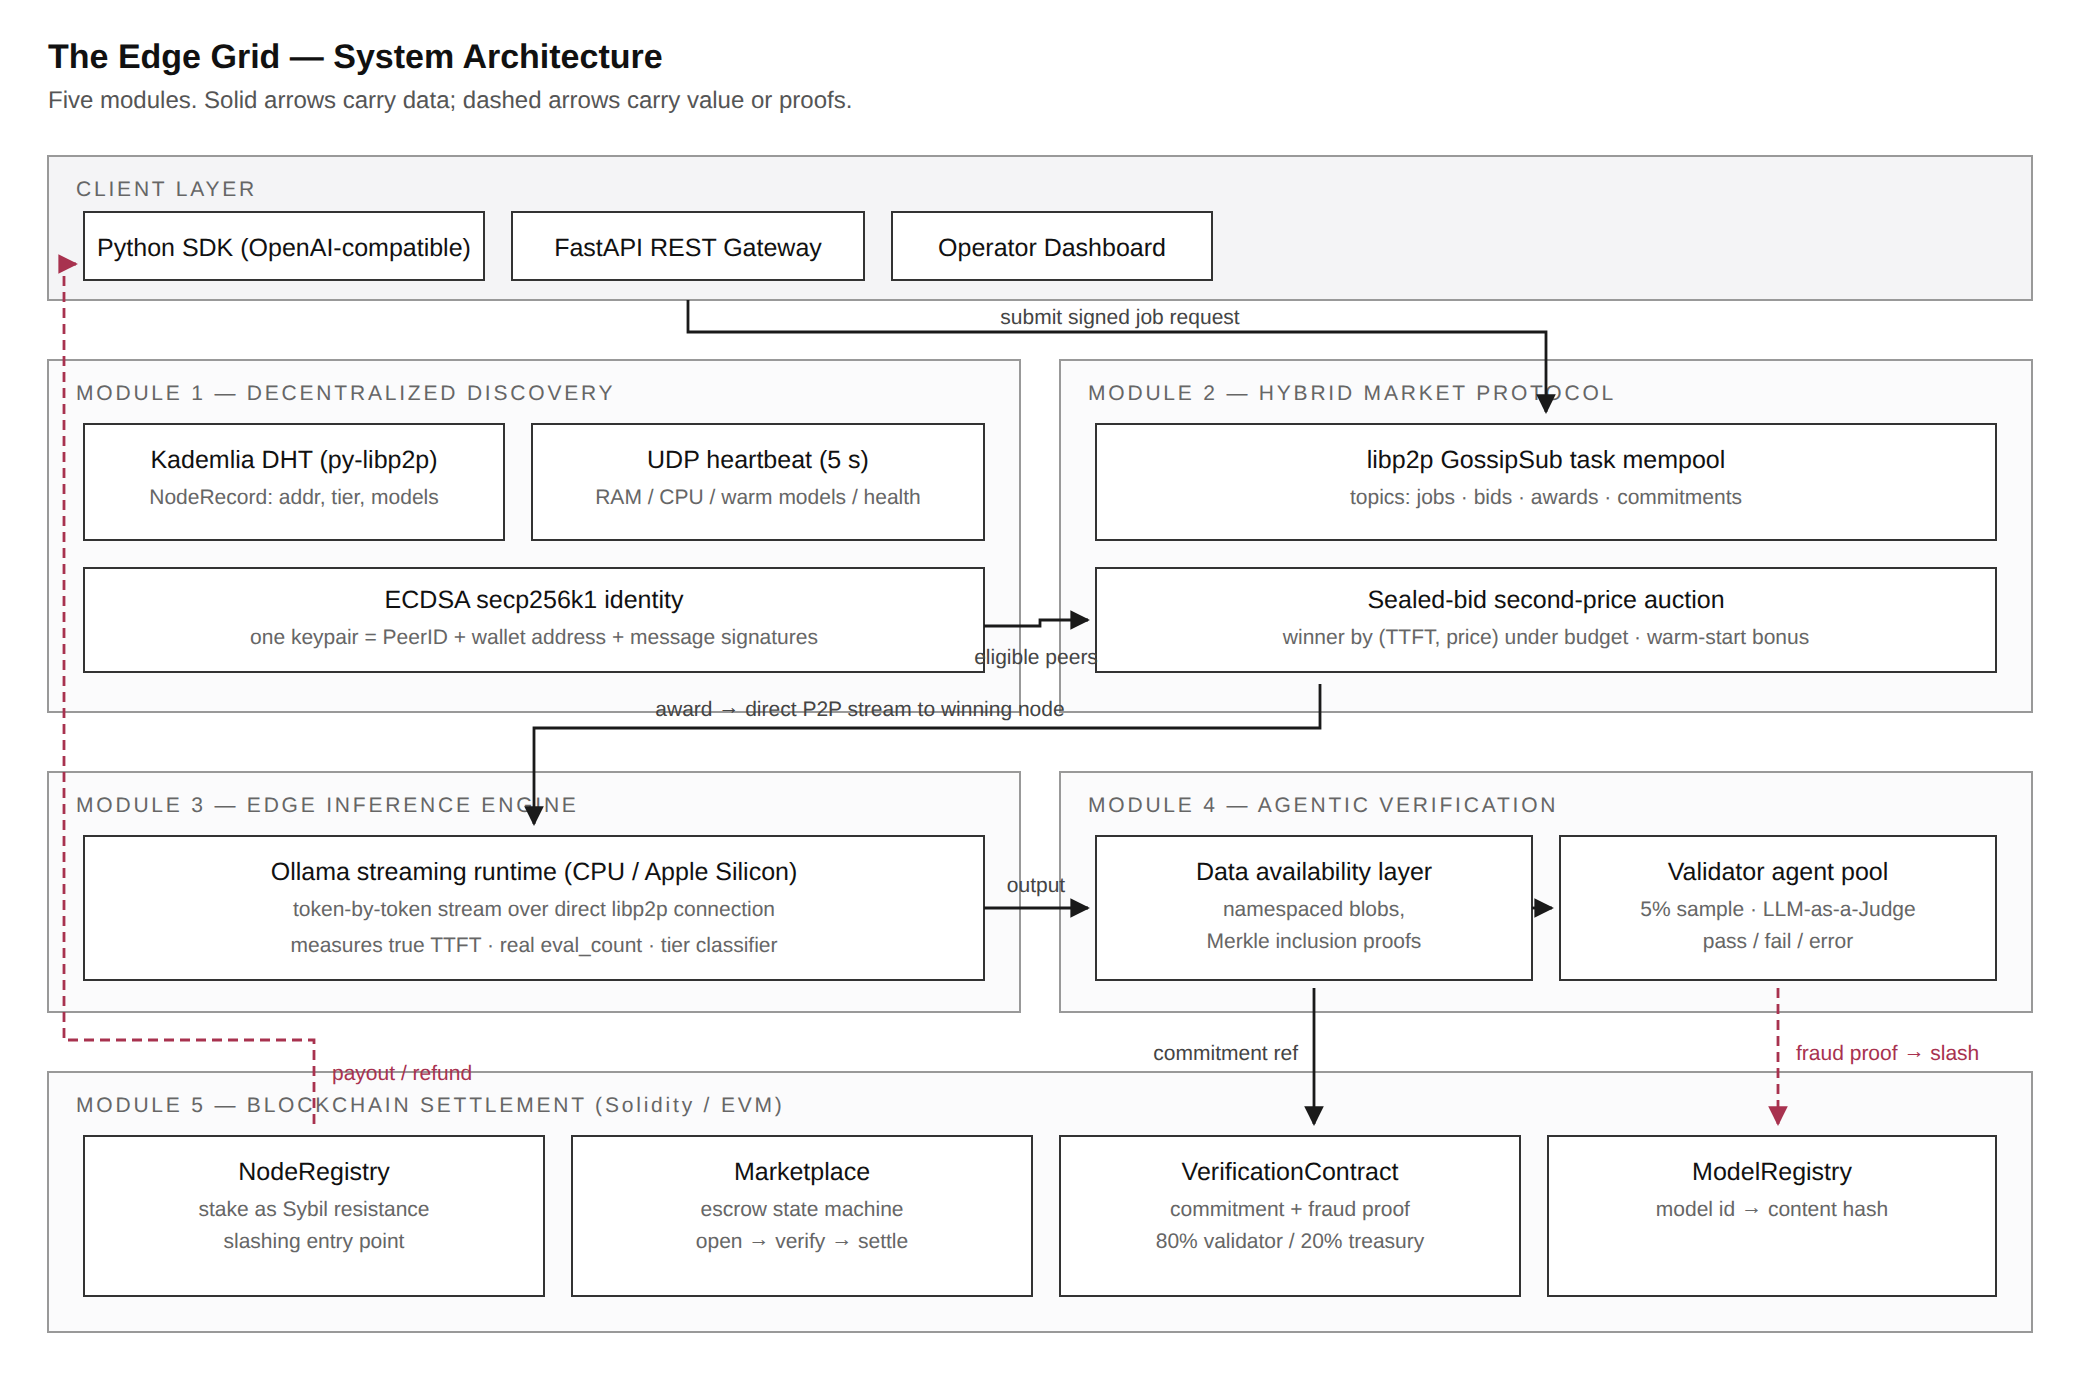
\includegraphics[width=0.92\textwidth]{architecture.png}
\caption{System architecture: a client layer and five modules. Solid arrows carry data; dashed
arrows carry value or proofs.}
\label{fig:arch}
\end{figure*}

\textbf{System model.} Four roles (requesters, providers, validators, and a settlement layer)
compose a five-stage pipeline (discovery, market, inference, verification, settlement)
communicating through a fixed message contract (Fig.~\ref{fig:arch}).

\textbf{Threat model.} Cheating providers are split into two trust classes: an output
inconsistent with what was committed on chain is \emph{provably} dishonest (a hash mismatch,
checkable by anyone); an output that is faithfully delivered but factually wrong requires a judge,
whose error rate is an irreducible cost. Colluding provider/validator pairs are mitigated
structurally: deterministic, unpredictable sampling means a provider cannot know which jobs will be
audited, but validator collusion at scale is \textbf{not} claimed solved. Sybil resistance is
economic (identity multiplication is cheap, but acting under an identity without stake is not)
rather than identity-based, and its adequacy against a well-resourced adversary is an open
question. Latency misreporting is deferred to the general verification path rather than a
dedicated mechanism, a stated gap.

\textbf{Discovery and identity.} One secp256k1 keypair doubles as network identity and settlement
wallet. A slow-changing \textbf{capability record} (models served, tier, stake) propagates through
a DHT; a fast-changing \textbf{liveness signal} (reachability, which models are \emph{loaded and
ready}) propagates directly between peers. The two are kept separate because collapsing them
forces a choice between an expensive high-frequency DHT update and a stale signal that an auction
clearing in seconds cannot use.

\textbf{Market protocol.} A sealed-bid, second-price \emph{procurement} auction: providers bid the
price they want to be paid; the lowest eligible bid wins but is paid the second-lowest eligible
price, making truthful bidding dominant. Eligibility (tier, latency, price ceiling) is checked as
hard constraints before any price comparison. A warm-model discount is applied to \emph{ranking
score} only, never to payment, preserving individual rationality, because over realistic latency
budgets a cold provider's fixed load cost makes warmth closer to an eligibility condition than a
tradeable quality dimension (confirmed empirically in Section~\ref{sec:latency}).

\textbf{Inference contract.} A narrow, runtime-agnostic contract: stream tokens, report true
time-to-first-token (TTFT) and a real per-request token count, and report cold/warm state. A
provider that cannot report these honestly cannot participate.

\textbf{Verification protocol.} Every job is committed to a content-addressed store. A
deterministic-but-unpredictable sample is audited: first a purely mechanical check (does the
committed output match the store, under a Merkle proof requiring no model or judgment: a
\textbf{fraud proof}, treated as certain); only if that passes does one or more validators render
a semantic verdict, required to be one of three values (pass, fail, or \textbf{unavailable}), so a
judge outage is never conflated with either an acquittal or a slash. Validator \emph{diversity} is
recorded as a first-class property rather than assumed.

\begin{figure}[t]
\centering
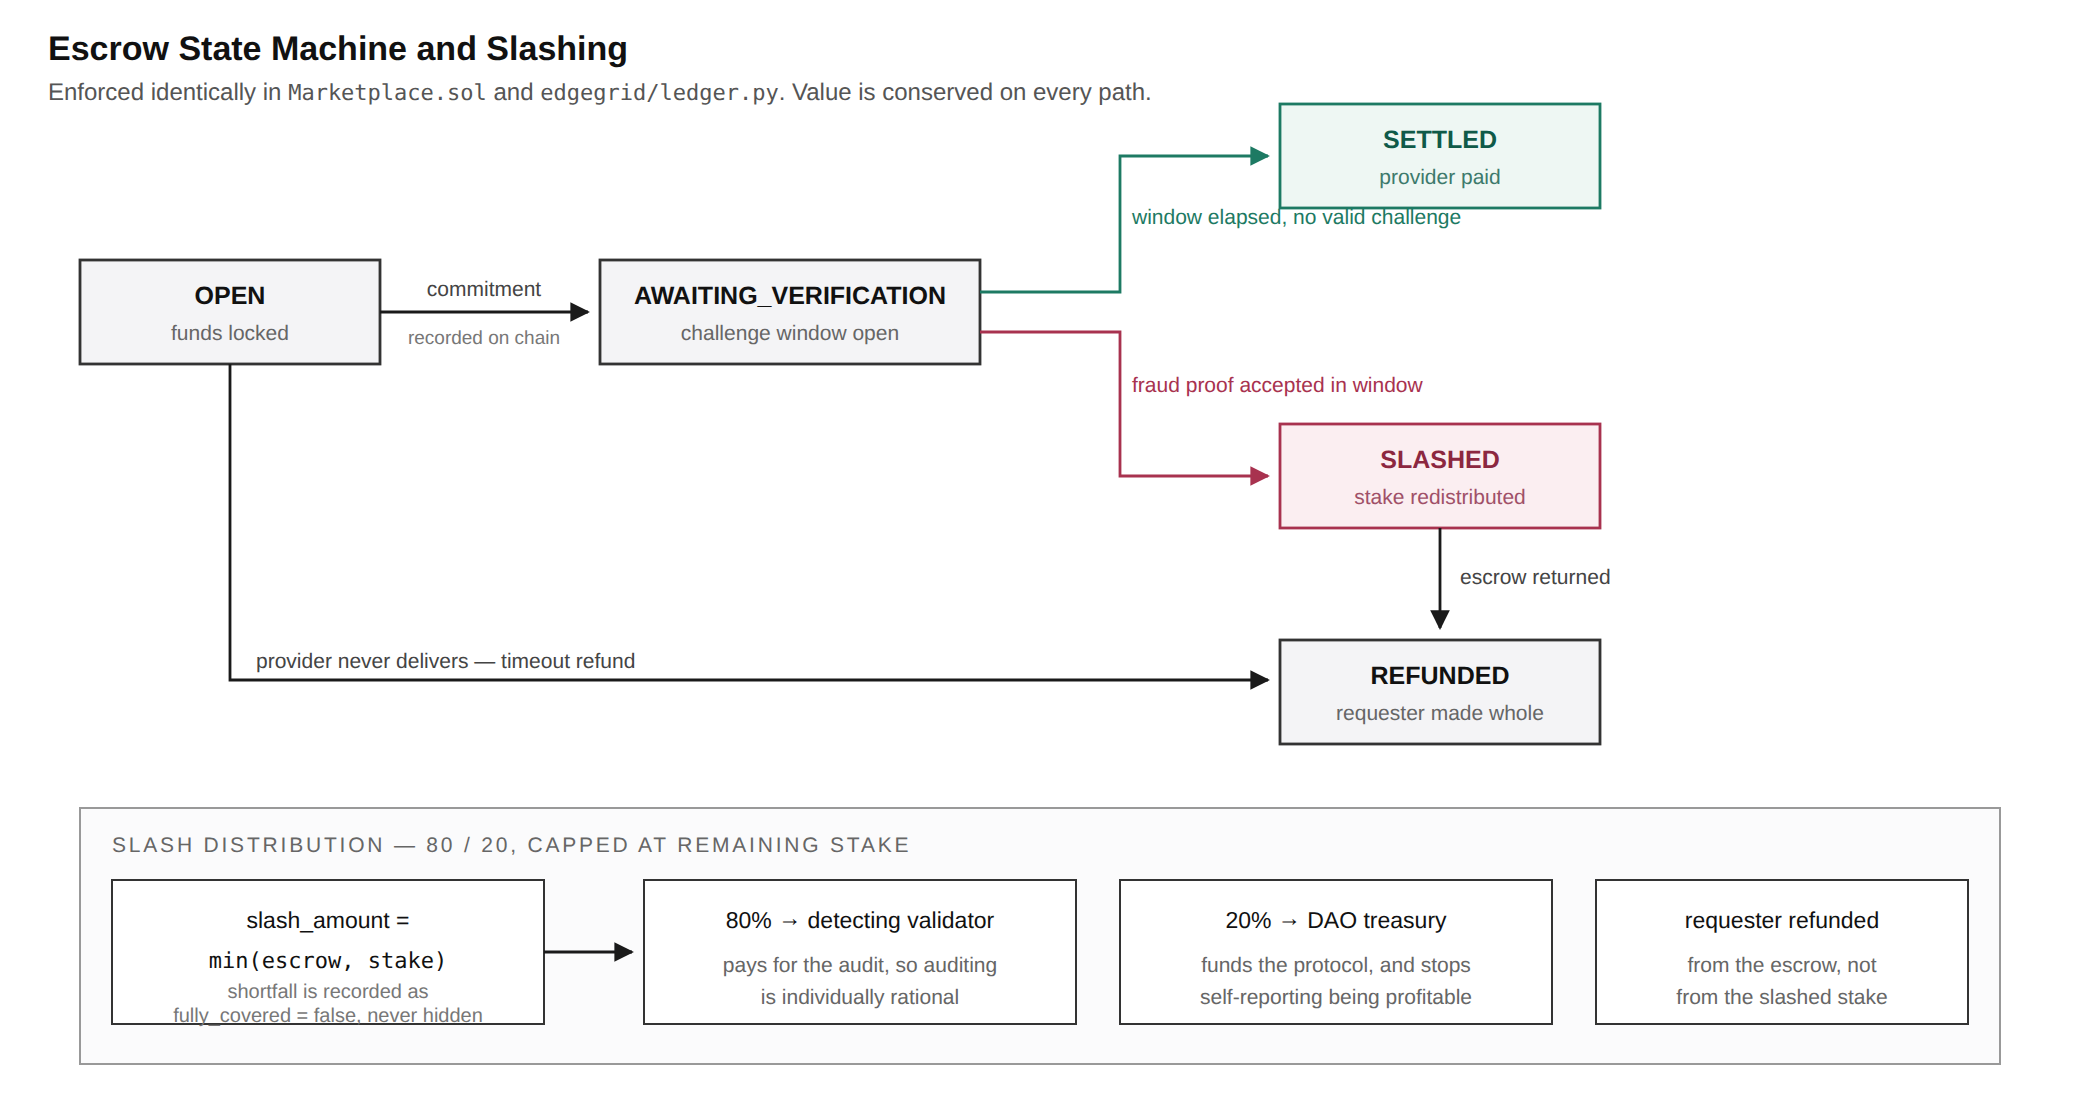
\includegraphics[width=\columnwidth]{settlement_states.png}
\caption{Escrow state machine and the 80/20 slash distribution, enforced identically in the
Solidity contracts and the Python ledger.}
\label{fig:settle}
\end{figure}

\textbf{Settlement.} A fixed challenge window follows commitment; uncontested release requires no
privileged party online. Confirmed fraud (proof or FAIL verdict) returns escrow to the requester
and slashes provider collateral 80/20 between reporter and treasury (Fig.~\ref{fig:settle}).
Withdrawn collateral stays slashable during an unbonding delay, closing a front-running window.

% ---------------------------------------------------------------------------
\section{Implementation}

Five cooperating tracks share one wire contract, in Python except settlement: discovery and market
over a Kademlia and GossipSub library (py-libp2p); inference against a streaming open-weight
runtime exposing token-level timing (Ollama, replaceable behind the same contract); settlement as
four Solidity contracts on a local development chain; and weight distribution against a real IPFS
daemon with client-side content-identifier recomputation (never trusting the daemon's own claim).
Every message carrying economic consequence is signed and independently re-verified.

\begin{table*}[t]
\caption{Design Versus Prototype}
\label{tab:proto}
\centering
\footnotesize
\begin{tabular}{P{2.4cm}P{3.6cm}P{3.6cm}P{6.2cm}}
\toprule
\textbf{Component} & \textbf{Prototype} & \textbf{Production target} & \textbf{Limitation left open}\\
\midrule
Settlement chain & Local single-node dev chain & Arbitrum Stylus rollup & No fee market, no finality delay; fraud-proof censorability untested\\
Data availability & Local Merkle-committed blob store & Celestia (DA sampling) & Binding is real; availability under deletion is not\\
Inference runtime & CPU-only, single 2B model & GPU-accelerated serving stack & No figure bears on GPU-tier economics\\
Verification judge & Small, locally hosted (deployed); larger, hosted (measured separately) & Locally hostable, adequately capable pool & Deployable configuration fails adversary-favored strategies; the configuration that succeeds is not edge-hostable\\
Economic stake & Test-denomination collateral & Real, market-priced & No conclusion about deterrent adequacy\\
\bottomrule
\end{tabular}
\end{table*}

Table~\ref{tab:proto} maps each component to its production target. Every experiment ran on one
host (16 cores, about 31\,GB RAM, no accelerator); the auction was also run in per-container network
namespaces with \texttt{tc netem}-injected link delay, isolating a per-peer link delay that a
shared-loopback topology cannot express. Every run writes a timestamped, never-overwritten
directory with a full configuration snapshot and git SHA; a component that cannot be reached raises
a named exception rather than returning a plausible-looking default.

% ---------------------------------------------------------------------------
\section{Evaluation}

\subsection{Latency}\label{sec:latency}

Warm TTFT: mean 609.6\,ms, median 587.9\,ms, p95 723.6\,ms ($n=20$; \textbf{all 20 under one
second}). Cold TTFT averaged 7{,}963.8\,ms against a paired warm 653.7\,ms, a
\textbf{12.18$\times$} ratio, attributable almost entirely to model \emph{load} time
(7{,}418\,ms cold vs.\ 568\,ms warm), not generation (Fig.~\ref{fig:ttft}). This is the direct
empirical justification for pricing warmth near eligibility rather than as a smooth quality
signal.

\begin{figure}[t]
\centering
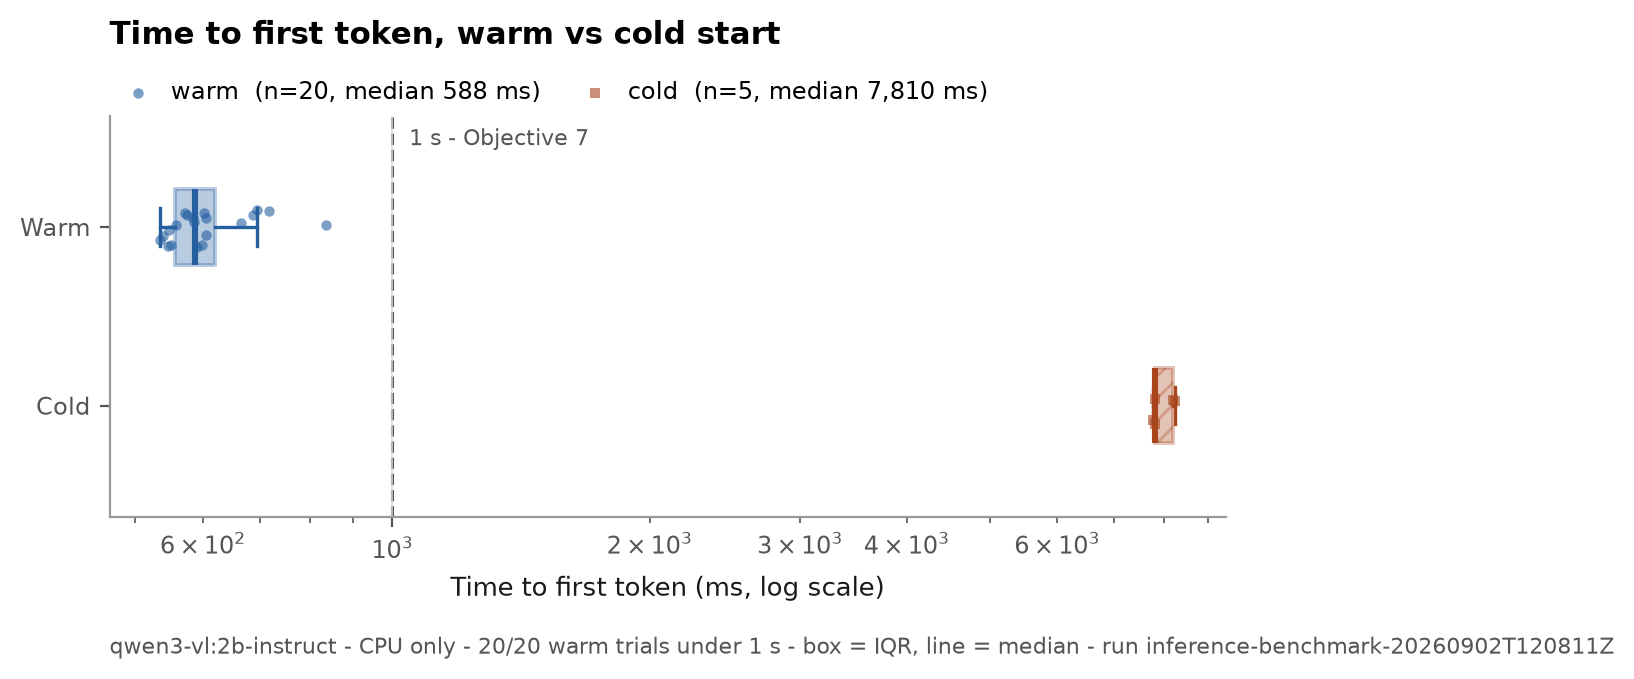
\includegraphics[width=\columnwidth]{fig_ttft.png}
\caption{Time to first token, warm versus cold start, on a logarithmic time axis.}
\label{fig:ttft}
\end{figure}

\subsection{Auction Convergence}\label{sec:auction}

Fifty-seven single-machine auctions (3, 4, and 5 nodes) cleared with zero failures.
Broadcast-to-award was pinned at about 2{,}008\,ms by the fixed bid window and is not a scaling
signal; the un-pinned bid-arrival times carry the real signal, with last-bid latency rising from
21.3 to 32.6 to 36.7\,ms. Under container network namespaces with injected one-way link delay of
0, 10, 25, and 50\,ms, first-bid arrival rose from 6.0 to 44.5, 71.0, and 114.0\,ms, close to but
above a bare round-trip reference line: roughly \textbf{2.06\,ms of added delay per ms injected},
consistent with GossipSub relaying through a third peer on some messages.

\subsection{Verification Accuracy}\label{sec:verif}

We ran 100 trials (80 fraudulent across four corruption strategies, 20 honest) on
TruthfulQA~\cite{truthfulqa}. The judge failed \textbf{none} of the 20 honest answers (100\%
precision, 0\% false-positive rate). This is a corrected result: an earlier run had shown a 75\%
false-positive rate, since diagnosed as a fault in the honest-answer \emph{generator}, not the
judge. \textbf{Overall recall was 65\%, sharply bimodal}: 100\% and 95\% on off-topic and
fabricated-entity fraud, versus \textbf{35\% and 30\%} on plausible-substitution and negation
fraud (Fig.~\ref{fig:verif}). The missed fraud was scored \emph{confidently} (3.80--4.05 out of 5
against a pass threshold of 3), not near the threshold, which rules out raising the threshold as a
fix.

\begin{figure}[t]
\centering
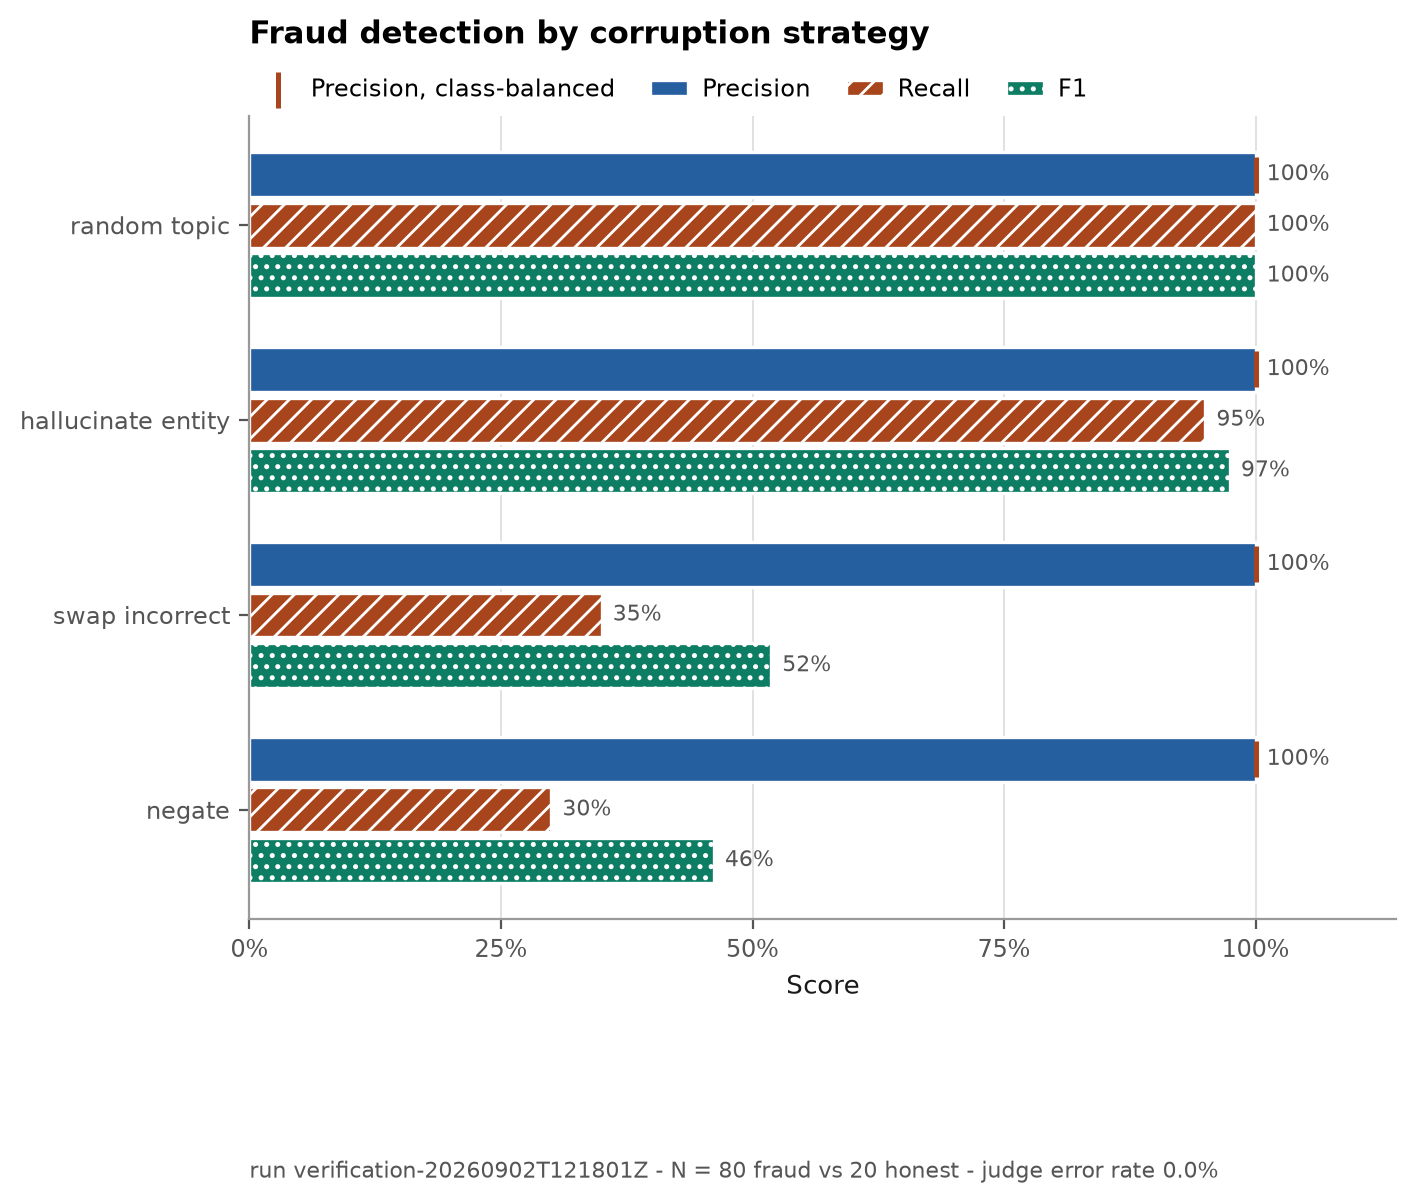
\includegraphics[width=\columnwidth]{fig_verification.png}
\caption{Fraud detection by corruption strategy: precision, recall, and F1.}
\label{fig:verif}
\end{figure}

\textbf{Capability, not lineage.} We re-judged the same 80 strings with larger hosted models. A
judge about 13$\times$ larger from the \emph{same family} as the provider model recovered negation
recall to 100\% (98\% overall); a judge from an \emph{unrelated} family reached 100\% and 90\% on
the two subtle strategies (96\% overall). This refutes our initial hypothesis that lineage, not
capability, explained the gap. Under majority-vote quorum across all four panel members, recall
reached 97\% at a \textbf{7\%} false-positive rate, versus 26\% and 16\% for the two individual
complete members (Fig.~\ref{fig:panel}). This directly supports quorum aggregation, qualified by
the fact that two of the four members were rate-limited by their free-tier APIs and returned
usable verdicts on fewer than 20\% of items, so the capability-versus-lineage contrast rests on one
same-family and one unrelated-family judge. Judge self-consistency under paraphrase (small judge,
8 questions) showed a \textbf{25\%} verdict-flip rate on reworded claims.

\begin{figure}[t]
\centering
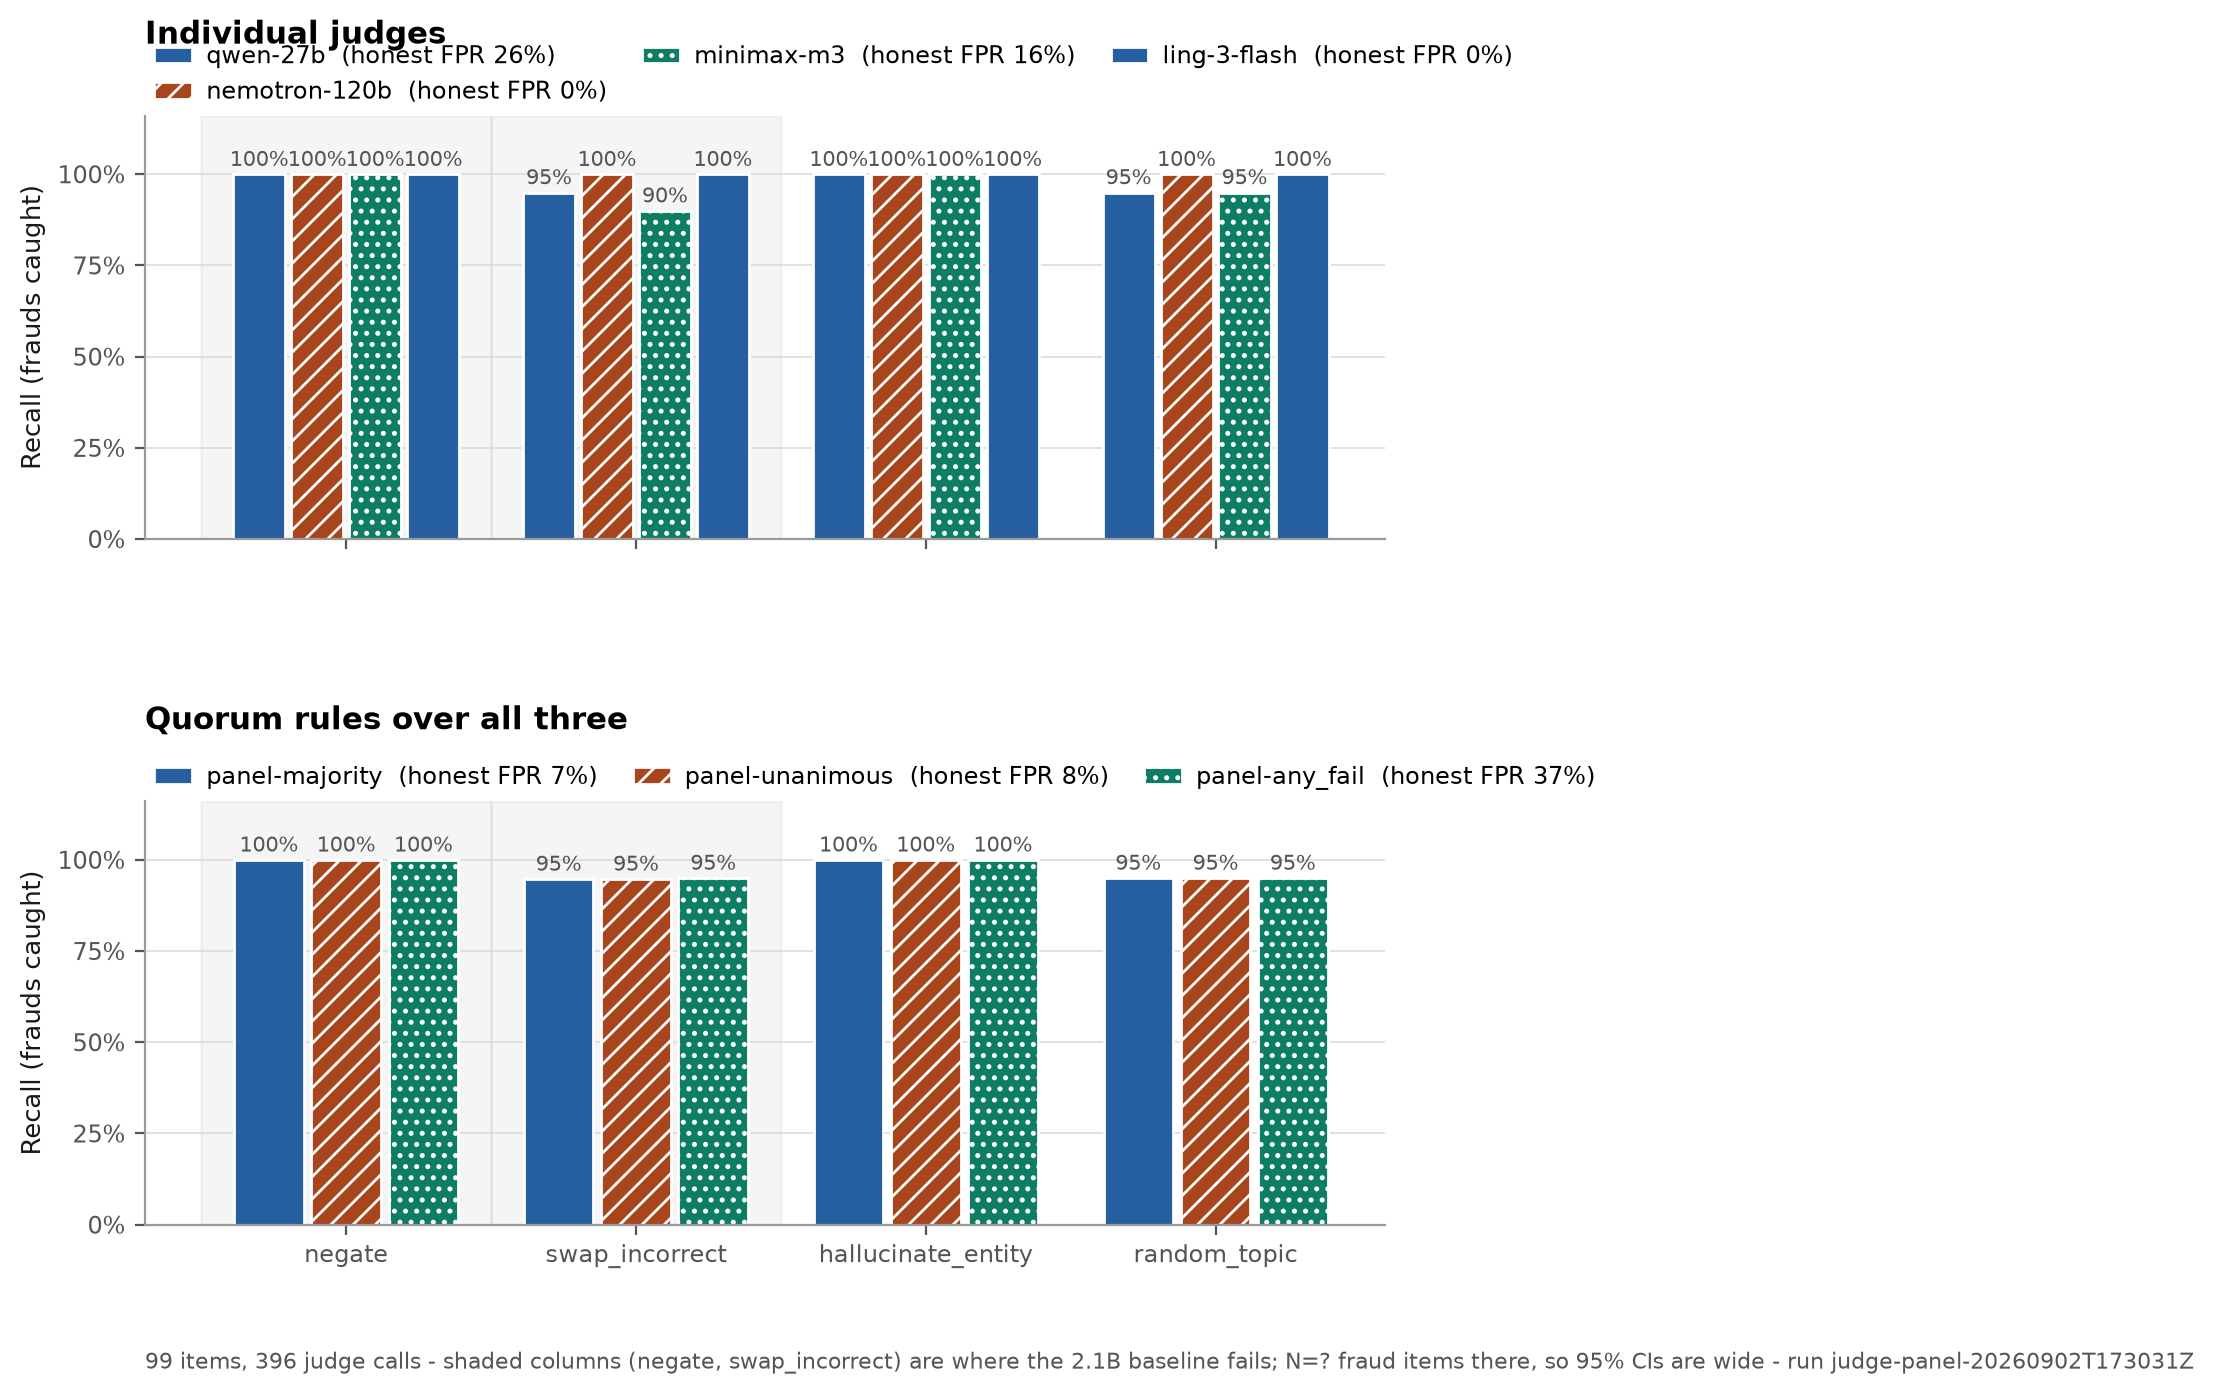
\includegraphics[width=\columnwidth]{fig_judge_panel.png}
\caption{Recall by corruption strategy for each judge and quorum rule.}
\label{fig:panel}
\end{figure}

\subsection{Weight Distribution and Cost}

Five artefacts (64\,KiB to 48\,MiB) were distributed through a real IPFS daemon: cold fetch took
6.6--317.5\,ms and warm (cached) fetch under about 1.5\,ms, speedups of
\textbf{12.3$\times$--895.8$\times$}, with the content identifier independently recomputed on every
fetch; three tampering scenarios were correctly rejected against one honest control accepted.
Three on-chain settlements (honest release, fraud-proof slash, verdict slash) all resolved
correctly with an exact 80/20 split and exact value conservation. Gas ranged from 32{,}317
(withdrawal) to 221{,}353 (the trustless fraud proof, which is the best value in the system since it
requires no model). The composed cost is \textbf{\$0.00115} per 1{,}000 tokens (verification
4.8\% of that) against a \textbf{\$0.002} centralized baseline; this is a notional-rate cost
\emph{model}, not a market observation.

% ---------------------------------------------------------------------------
\section{Discussion}

The prototype shows that the five-stage pipeline of Section~\ref{sec:design} holds together as a
running system rather than as a set of separately plausible components: a real signed job travels
from broadcast, through a real gossip-mesh auction that clears correctly and is individually
rational on every measured award, through a real streaming inference call whose warm latency
clears a sub-second target, through a real content-addressed weight fetch a node can verify
without trusting its source, through a real Merkle-committed data-availability check, to a real
on-chain escrow that resolves correctly down all three of its state-machine paths and conserves
value exactly. That composition, not any individual mechanism (all of which are prior art,
Section~II), is what this evaluation is able to support at small scale.

What it does not show is comparably important. Every network measurement, including the auction
under injected latency, ran on one physical kernel; nothing here establishes behavior across real
wide-area links, NAT traversal, packet loss, or peer churn; three to five nodes cannot establish a
scaling law; gas figures are priced against no fee market or contention; and staked collateral in
every run is a test value with no real cost to lose, so no conclusion follows about deterrent
adequacy. The mechanism's incentive-compatibility argument is a property of its construction, not
something measured here.

The \textbf{central finding} is not a number but a corrected explanation. It would have been easy
to conclude that a same-family judge inherits the fraud-generating model's blind spots, making
diversity the fix; the panel experiment instead indicates that capability, not lineage, closed the
gap. A second, general finding travels alongside it: \textbf{every false-positive rate in this
evaluation is confounded by the fallibility of whichever model generated the ``honest''
control}, a milder recurrence of the exact failure that produced the earlier 75\% false-positive
result. Judge inconsistency under paraphrase compounds both: a single verdict is not a stable basis
for an irreversible slash. Automated, on-chain slashing driven by an LLM's judgment therefore makes
\emph{which judge, at what capability, under what quorum rule} a safety-critical configuration
choice, not a tuning parameter.

% ---------------------------------------------------------------------------
\section{Conclusion and Future Work}

Five mechanisms studied separately in prior literature (peer-to-peer discovery, an auction market,
streaming edge inference, two-tier verification, and staked settlement) compose into one measured,
end-to-end pipeline. The prototype's most useful result is a refuted hypothesis: the verification
layer's failure on adversary-favored fraud tracks judge capability, not lineage, correcting our own
initial explanation rather than confirming it.

\textbf{Future work}, each item tied to a named limitation: (1)~a genuine multi-machine deployment,
the largest unaddressed threat, since every network measurement here shares one kernel; (2)~a
capability-adequate, \emph{edge-hostable} judge, since the configuration that closes the recall gap
is not deployable on the hardware tier this network targets; (3)~a human-adjudicated honest control
set, the precondition for any clean judge-precision measurement; (4)~the production substitutions
of Table~\ref{tab:proto} (Celestia, a real rollup, GPU-accelerated serving, a public IPFS swarm);
(5)~an adaptive adversary that reallocates toward undetected fraud strategies; and
(6)~zero-knowledge verification of model execution, which would make judge capability moot but
remains orders of magnitude too expensive for a sub-second latency target today.

\section*{Acknowledgment}

The authors thank their project guide, Dr.\ Savita Choudhary, Professor and Head, Department of
CSE (IoT, Cyber-Security and Blockchain Technology), Sir M. Visvesvaraya Institute of Technology,
for guidance throughout this work.

% ---------------------------------------------------------------------------
\begin{thebibliography}{00}
\bibitem{bittensor} E. Lui and J. Sun, ``Bittensor protocol: The Bitcoin in decentralized AI?'' in \emph{Proc. MARBLE 2025}, Springer, pp.~145--165.
\bibitem{akash} G. Osuri and A. Bozanich, ``AKT: Akash network token \& mining economics,'' Whitepaper, 2020.
\bibitem{golem} Golem Factory GmbH, ``The Golem project: Crowdfunding whitepaper,'' 2016.
\bibitem{gensyn} Gensyn AI Ltd., ``Gensyn litepaper,'' 2022.
\bibitem{morpheus} Morpheus, Trinity, and Neo, ``Morpheus: A network for powering smart agents,'' Whitepaper, 2023.
\bibitem{morpheusnode} MorpheusAIs, \emph{Morpheus-Lumerin-Node} [Software], 2024--.
\bibitem{dgrid} DGrid.AI, ``DGrid AI: The decentralized AI inference network,'' Litepaper, 2025.
\bibitem{parallax} C. Tong \emph{et al.}, ``Parallax: Efficient LLM inference service over decentralized environment,'' arXiv:2509.26182, 2025.
\bibitem{polylink} H. Liu \emph{et al.}, ``PolyLink: A blockchain based decentralized edge AI platform for LLM inference,'' in \emph{Proc. IEEE Blockchain 2025}, pp.~101--108.
\bibitem{albassam} M. Al-Bassam \emph{et al.}, ``Fraud and data availability proofs: Detecting invalid blocks in light clients,'' in \emph{Proc. FC 2021}, LNCS 12675, pp.~279--298.
\bibitem{arbitrum} L. Bousfield \emph{et al.}, ``Arbitrum Nitro: A second-generation optimistic rollup,'' Offchain Labs, Whitepaper, 2022.
\bibitem{truebit} J. Teutsch and C. Reitwie{\ss}ner, ``A scalable verification solution for blockchains,'' TrueBit Whitepaper, 2017.
\bibitem{mtbench} L. Zheng \emph{et al.}, ``Judging LLM-as-a-Judge with MT-Bench and Chatbot Arena,'' in \emph{Proc. NeurIPS 2023}.
\bibitem{arena} W.-L. Chiang \emph{et al.}, ``Chatbot Arena: An open platform for evaluating LLMs by human preference,'' in \emph{Proc. ICML 2024}, PMLR 235.
\bibitem{truthfulqa} S. Lin, J. Hilton, and O. Evans, ``TruthfulQA: Measuring how models mimic human falsehoods,'' in \emph{Proc. ACL 2022}, pp.~3214--3252.
\bibitem{petals} A. Borzunov \emph{et al.}, ``Petals: Collaborative inference and fine-tuning of large models,'' in \emph{Proc. ACL 2023 (System Demonstrations)}, pp.~558--568.
\bibitem{petals2} A. Borzunov \emph{et al.}, ``Distributed inference and fine-tuning of large language models over the Internet,'' in \emph{Proc. NeurIPS 2023}.
\bibitem{navigator} Y. Yang \emph{et al.}, ``Navigator: A decentralized scheduler for latency-sensitive AI workflows,'' in \emph{Proc. IEEE EDGE 2024}, pp.~35--47.
\end{thebibliography}

\end{document}
